%%%%%%%%%%%%%%%%%%%%%%%%%%%%%%%%%%%%%%%%%%%%%%%%%%%%%%%%%%%%%%%%%%%%%%%%%%%%%%%%%%%%%%
% This LaTeX file was prepared by:
%       Rajat Subhra Chakraborty
%       Assistant Professor
%       Dept. of Computer Science and Engineering
%       IIT Kharagpur
%       Kharagpur, India - 721302
%       E-mail: rschakraborty@cse.iitkgp.ernet.in
%       Last Modified: 18th April, 2014
%%%%%%%%%%%%%%%%%%%%%%%%%%%%%%%%%%%%%%%%%%%%%%%%%%%%%%%%%%%%%%%%%%%%%%%%%%%%%%%%%%%%%%
\documentclass{article}
\usepackage[pdftex]{color,graphicx}
\usepackage{amsmath}
\usepackage{amssymb}
\usepackage{enumerate}
\usepackage{syntonly}
\usepackage{multicol}
\usepackage{eqnarray}
\usepackage{exam}

\paper{CS60004}  % <- do not include FC, FT etc
%\version{0}                     % <- for multiple choice exams
\subject{CS60004: Hardware Security}
\title{End--semester Examination}
\time{3}                      % <- number of hours: default is three
\semester{Spring}
\year{2016}                     % <- default is the current year
%\campus{City}
\fullmarks{50}
\note{\textbf{ANSWER ANY 5 QUESTIONS.} You can attempt the questions in any order, but preferably all the sub-parts 
of an attempted question should be solved in one place.}

\begin{document}

\begin{questions}
\question Consider the AES-128 iterated architecture as shown in 
{\bf Fig.~\ref{loopAES1}}. The inputs plaintext and the key are stored 
in the D-FlipFlops, marked as DFF. There are few intermediate 
FlipFlops (DFF\_1, DFF\_2, DFF\_3), 
and the ciphertext is stored in another output DFF. The time delays 
for the blocks are: SubBytes ($T_{SB}$), ShiftRows ($T_{SR}$), 
MixColumns ($T_{MC}$), AddRoundKey ($T_{AR}$), Multiplexer ($T_{MUX}$), 
and Demultiplexer ($T_{DEMUX}$). Ignore the hardware cost for the 
Key Scheduler and also its effect on the timing, as the encryption key is 
fixed for a long time. Answer the following questions in this regard:
\begin{enumerate}
\item Assuming, the path delays as above, estimate the critical 
path delay of the architecture. Remember critical path means the longest combinational path delay 
from register to register. \marks{3}
\item A designer wishes to make an alternative architecture in order to reduce 
the area overhead. Suggest an alternate design by drawing the modified architecture. \marks{4}
\item Estimate the critical path delay of the modified architecture. \marks{3} 
\end{enumerate} 


\begin{figure}[h]
\centering
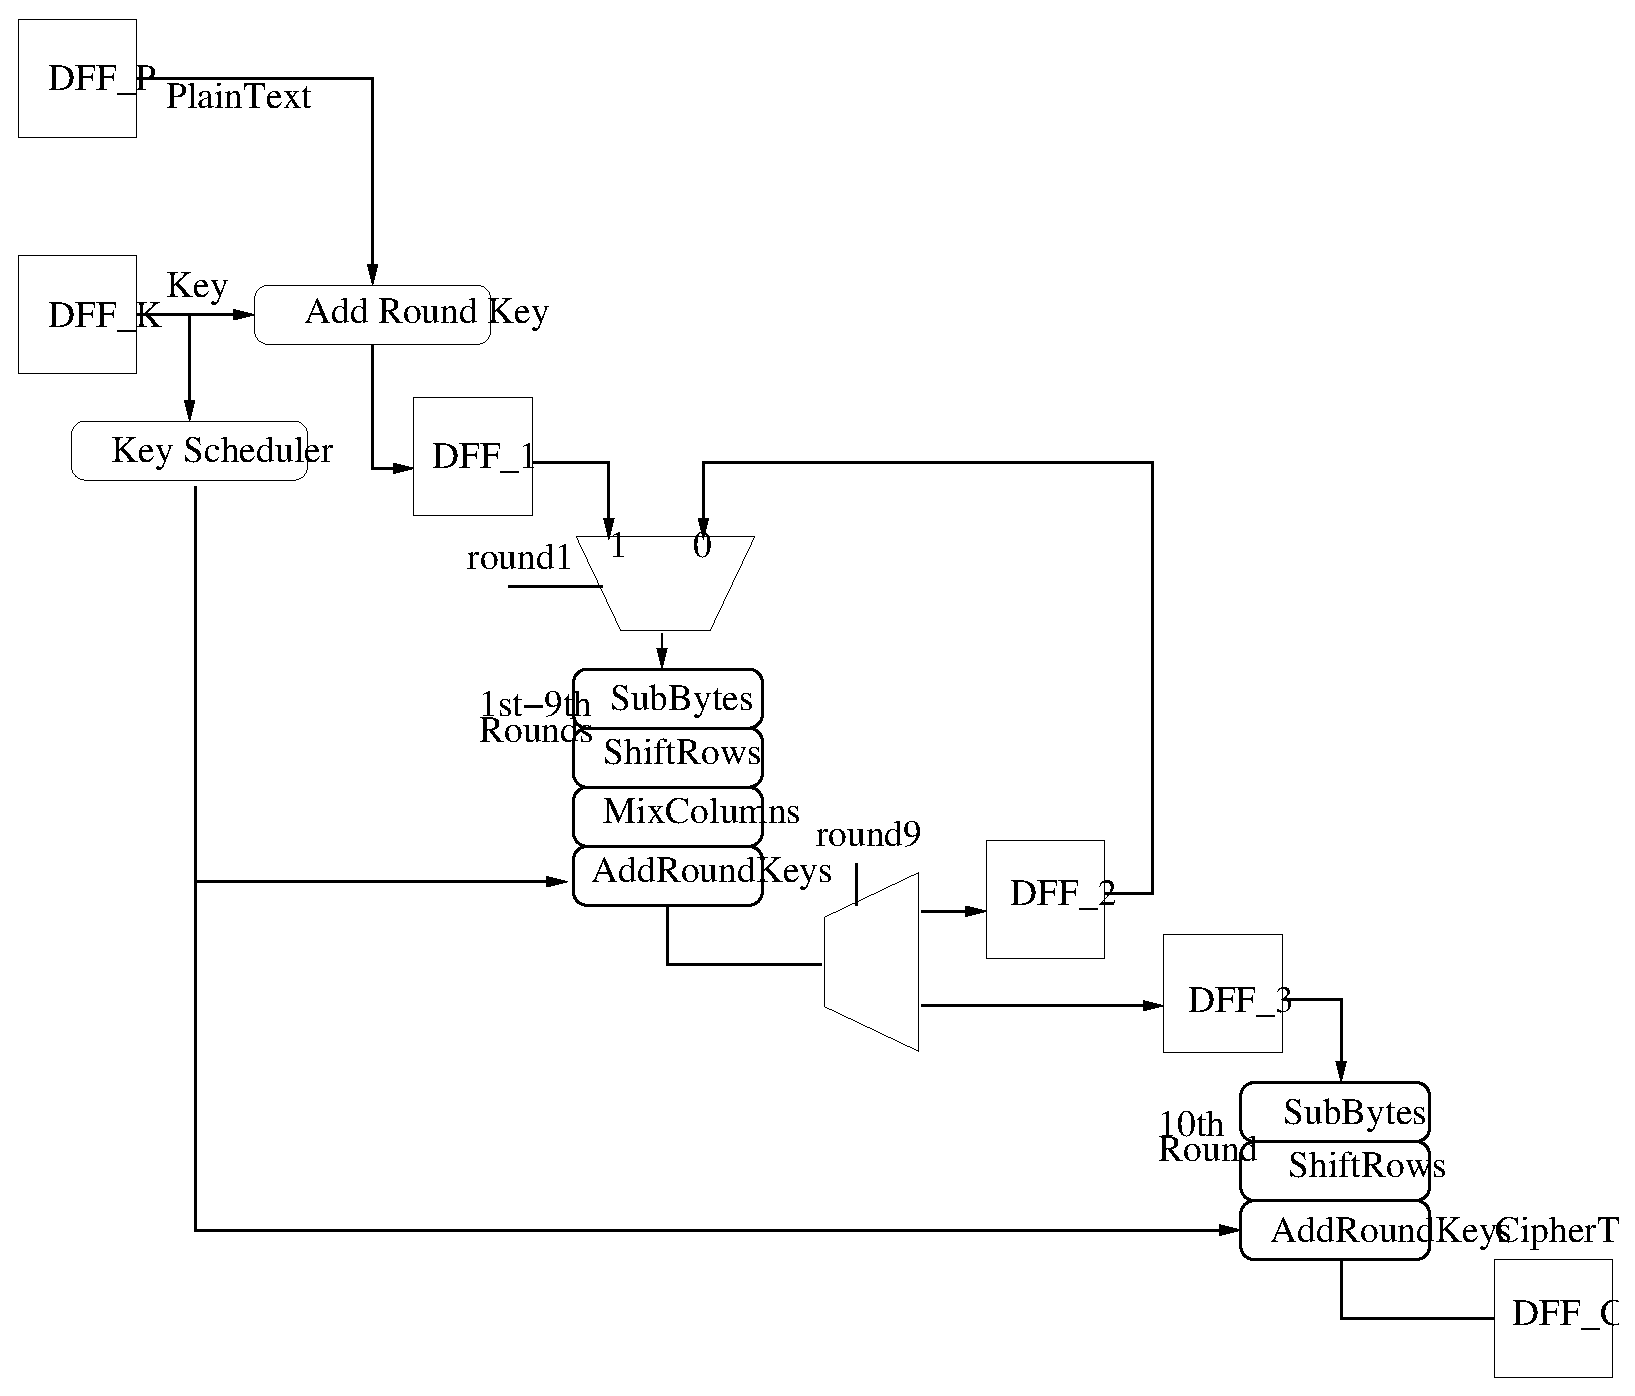
\includegraphics[width=4in]{loopAES}
%\epsfig{file= Images/isgreater.jpg, width=3.0in}
\caption{An Iterated Architecture for AES-128 Encryption}
\label{loopAES1}
\end{figure}


\question A student named {\em Complex} wants to develop an efficient architecture for a 
$GF(2^4)$ inverse. For this first he wants to obtain an isomorphic mapping 
between the fields $GF(2^4)$ and $GF(2^2)^2$. Assume 
that the primitive polynomial of $GF(2^4)$ is $R(Z)=Z^4+Z+1$, 
$GF(2^2)$ is $Q(Y)=Y^2+Y+1$, while for $GF(2^2)^2$ the 
primitive polynomial is $P(X)=X^2+X+\{2\}$, where 
$\{2\}\in GF(2^2)$. 

His friend {\em KnowsAll} suggests two possible options for 
maps from $GF(2^4)$ to $GF(2^2)^2$:
 
{\bf Option 1:}$\{02\}\rightarrow \{04\}$, 
{\bf Option 2:}$\{02\}\rightarrow \{32\}$. 

Answer the following questions in this regard:
\begin{enumerate}
\item Argue about the correctness of both the mappings, as 
in Options 1 and 2. \marks{4}
\item For the valid options, derive the transformation matrix 
from $GF(2^4)\rightarrow GF((2^2))^2$. \marks{3}
\item Draw an efficient inversion architecture for an element 
in $GF(2^4)$ using the above transformation(s). Derivations must be shown for 
credit. \marks{3}
\end{enumerate} 



\question 
Consider a round of a block cipher as depicted in {\bf Fig.~\ref{Speck}} which has overall $T$ rounds. 
The rounds are indexed by $i$, where $1 \leq i \leq T$ and each block is of $2n$ bits, where each half is of 
$n$ bits. Each round 
is denoted as $R_{k^i}(x_{i},y_{i})=(x_{i+1},y_{i+1})=((S^{-a}(x^i)+y^i)\oplus k^i,S^b(y^i)\oplus (S^{-a}(x^i)+y^i)\oplus k^i)$, 
where $k^i$ is the round key also of size $n$ bits. The transformation $S^{-a}(x)$ indicates a cyclic right shift 
of the $n$ bit word $x$ by $a$ bits, while the transformation $S^b(x)$ denotes a cyclic left shift 
of the $n$ bit word by $b$ bits. The $n$ bit word $x$ is stored as 
$(x_{n-1},\cdots,x_0)$. 


An attacker named {\em Captain Speck} has an embedded device which implements the above cipher with the key internal to the hardware. 
The attacker has access to the input plaintext and the ciphertext, which are denoted as $(x_1,y_1)$ and $(x_{T+1},y_{T+1})$ 
respectively. He has the ability to inject {\bf bit} faults in the registers and he attempts to use it to break 
the cipher. Help him to do so by answering the following questions:
\begin{enumerate}
\item If the attacker induces a bit fault in the register $y^T$ when 
the last round is being 
operated, show that the attacker can also ascertain which bit is faulted 
from the ciphertexts.
\marks{3}

\item For the last round of the cipher prove the equation:
\begin{eqnarray*}
k_j^{T} &=& x_{(j+a)\%n}^T \oplus (y^{T+1} \oplus x^{T+1})_{(j+b)\%n}\oplus c_j \oplus x_j^{T+1}
\end{eqnarray*}
Here, for an $n$-bit word $x^T$, $x_j^T$ denotes the $j$-th bit of the word and $c_j$ is the 
$j$-th bit of the carry generated ie the carry input to the $j$-th bit position. 
\marks{3}

\item Assume that the fault is induced in the $0^{th}$ bit 
of the register $y^T$, ie $y_0^T$ when the last 
round is operated by the hardware. Show how can the attacker can retrieve the 
$0$-th key bit of the last round, ie. $k_0^T$. \marks{4}

{\bf {\em HINT for part (c): } Prove first that $(x^{T+1} \oplus x^{(T+1)*})_0=1$, where $x^{(T+1)*}$ corresponds to 
left part of the faulty ciphertext. Then use the Hamming Weight of  
$(x^{T+1} \oplus x^{(T+1)*})$.}
\end{enumerate}


\begin{figure}[h]
\centering
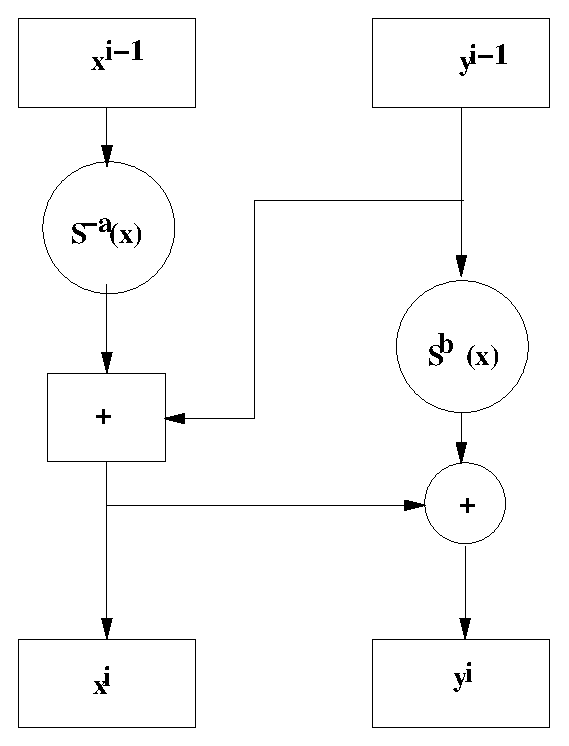
\includegraphics[width=2in]{Speck}
%\epsfig{file= Images/isgreater.jpg, width=3.0in}
\caption{Last Round of Cipher Speck}
\label{Speck}
\end{figure}

\question Consider the following program which sorts an array of $N$ numbers that are  
arranged according to a {\em secret file}. The output of the program is the sorted array. 
\begin{verbatim}
  #define N  5
  swapper(int *A){
     int i, j, tmp;
     int B[N];

     /* 1. Read a random permutation of {1,2,3,..., N} from file "Secret" into array B */
     /* 2. Fill N random integers into array A such that 
           A[i] is the B[i]-th smallest element in the array */
     /*   (Assume that operations 1 and 2 execute in constant time) */

     /* 3. Sort A */
     for(i=0; i<N-1; ++i){
         for(j=i+1; j<N; ++j){
            if (A[i] > A[j]){
               tmp = A[i];
               A[i] = A[j];
               A[j] = tmp;
            }
         }
     }
  
  }
\end{verbatim}

For instance, if 
\begin{verbatim}
   B = {3, 1, 2, 5, 4}
   choose 5 random integers say 10, 54, 22, 64, 33
   A = {33, 10, 22, 64, 54}
   Note, that 33 is the 3rd smallest element in A, 
              10 is the 1st smallest element in A,
              22 is the 2nd smallest element in A, etc.
\end{verbatim}
Describe a way that you can determine B using timing channels.
You have black box access to the function and are allowed to invoke it as many times as needed. \\

{\bf {\em HINT : } Connect this to Kocher's timing attack on RSA by noting that every swap results in a different 
timing from no swapping. Note that the attacker needs to obtain the 
array arrangement $A$ which is input to Step 3 of the above code. In the example, if the attacker is able to 
obtain the value of $A = \{33, 10, 22, 64, 54\}$, B is revealed.}

\marks{10}


\question {\em Prof No Fault} wants to design a counter-measure against fault injection based attacks on AES. 
He suggests to use a time redundancy based defence mechanism. The fault values of the AES output can be 
considered to form a fault space $F=\{f_1,f_2,\cdots,f_{2^{128}}\}$. Let $p_i$ be the 
occurrence of the fault $f_i$, where $1 \leq i \leq 2^{128}$, ie. $p_i=Pr[F=f_i]$. We 
denote $P$ as the probability distribution $\{p_1,p_2,\cdots,p_{2^{128}}\}$, 
where $\Sigma_{i=1}^{2^{128}}p_i=1$. However attacker {\em Hell Bent} wants to defeat the 
countermeasure by injecting two faults, in both the actual and redundant computations.

Answer the questions regarding the time redundancy countermeasure as follows:
\begin{enumerate}
\item Compute the success probability of {\em Hell Bent}, $\tilde{p}$, when the fault probability distribution is 
uniform, ie. $p_i=1/2^{128}$, $\forall i$.
\marks{4}

\item {\em Hell Bent} develops a new fault injection technique where the fault probability distribution is not 
uniform or is biased with a variance, {\em Var}. 
Show that to the aghast of {\em Prof No Fault} now the 
success probability of {\em Hell Bent} 
increases to $\tilde{p}=2^{128}(Var) + {1 \over 2^{128}}$.  \marks{6}
\end{enumerate}

\question Consider an $\tau$-variate leakage model for a hardware implementation of a block cipher, where the leakages of 
$\tau$ distinct time sample points are assumed to be dependent on a single intermediate 
value calculated during the execution of the underlying algorithm. Formally, 
assume for a time window, $0 \leq t < \tau$, 
$L_t=a_t(P+U+c)+N_t$, where $P$ is the hypothetical predicted leakage 
due to the target register (like an S-Box input in case of a standard DPA), 
$U$ is the leakage due to algorithmic noise, $c$ is the leakage due to 
control circuits, and $N_t$ is the electronic noise.

Assuming that both the algorithmic and electronic noise has zero means, and 
the variance of the electronic noise at each sample point 
is significantly higher than the signal variance, ie. 
$Var(E[L_t|P]) << Var(L_t-E[L_t|P])$, for $0 \leq t < \tau$, 
answer the following questions:
\begin{enumerate}
\item Prove that the SNR (Signal to Noise Ratio) of a sample 
point $t$, $\alpha(t)$ is proportional to the 
Squared Mean to Variance Ration, ie. $({\mu_{L_t} \over \sigma_{L_t}})^2$. 
Here, $\mu_{L_t}$ is the mean while $(\sigma_{L_t})^2$ is the Variance 
of the leakage $L_t$. \marks{5}

\item Prove that the Pearson's Correlation between the leakage 
at some sample point $L_t$ and the hypothetical predicted leakage for the 
correct key denoted by $k^*$, denoted by $\rho_{k^*}(t)$ is 
proportional to $({\mu_{L_t} \over \sigma_{L_t}})$. \marks{5}
\end{enumerate}


\end{questions}
\end{document}
